%Dokumentklasse

%draft als optionohne bilder für bessere performance
%\documentclass[a4paper,12pt,]{scrreprt}

%normal mit Bildern
\documentclass[
a4paper,
12pt,
draft=True]
{scrartcl}

%Section als Chapter
\RedeclareSectionCommand[%
%beforeskip = -1sp plus -1sp minus -1sp,% kleinster negativer Wert, um den Absatzeinzug nach der Überschrift zu verhindern.
afterskip = 1.5 \baselineskip plus -1sp minus 1sp,
font = \Huge,
]{section}

\usepackage[left= 3cm,right = 3cm, bottom = 3cm,top = 3cm]{geometry}
%\usepackage[onehalfspacing]{setspace}

% ============= Packages =============
% Dokumentinformationen
\usepackage[
pdftitle={Praktikum - Umwelttechnik},
pdfsubject={},
pdfauthor={Roman-Luca Zank},
pdfkeywords={},	
%Links nicht einrahmen
hidelinks
]{hyperref}

%nur Text zum prüfen des Umfangs

% Standard Packages
%\usepackage[bottom]{footmisc}
\usepackage[utf8]{inputenc}
\usepackage[ngerman]{babel}

\usepackage[T1]{fontenc}
%\usepackage{helvet}

%\renewcommand{\familydefault}{\sfdefault}

\usepackage{graphicx}
\graphicspath{{img/}}
\usepackage{mhchem}
\usepackage{fancyhdr}
\usepackage{lmodern}
\usepackage{color}
\usepackage{placeins}
\usepackage{booktabs}
\usepackage{caption}
\usepackage[list=true]{subcaption}
\usepackage{longtable}
\usepackage{tikz}
\usepackage{pgfplots}
\usepackage{lastpage}
%\usepackage{ulem}
\usepackage{mathtools}
\usepackage{adjustbox}
\usetikzlibrary{patterns}
\usepackage{pdfpages}
\usepackage{multirow}
%Einheitenpackage
\usepackage{siunitx}  
\sisetup{	locale = DE, 
	per-mode=fraction,
	inter-unit-product=\ensuremath{\cdot},
	detect-weight = true,
	quotient-mode=fraction
}
%neue Einheiten definieren
\DeclareSIUnit\xyz{xyz}	
\DeclareSIUnit\rpm{rpm}	
\DeclareSIUnit\mws{mWS}	
\DeclareSIUnit\degrees{^\circ}	

%Automatisch cdot statt *
\DeclareMathSymbol{*}{\mathbin}{symbols}{"01}


%Tabelle
\usepackage{tabularx}
\usepackage{tabulary}

%nur letzte Zeile der Gleichung nummerieren
\makeatletter
\def\Let@{\def\\{\notag\math@cr}}
\makeatother

% zusätzliche Schriftzeichen der American Mathematical Society
\usepackage{amsfonts}
\usepackage{amsmath}

%Abkürzungsverzeichnis
\usepackage{acronym}

%kein Abstand bei neuem Kapitel vom Seitenanfang
%\vspace*{2.3\baselineskip} = ORIGINAL
%\renewcommand*{\chapterheadstartvskip}{\vspace*{.0\baselineskip}}

%nicht einrücken nach Absatz
\setlength{\parindent}{0pt}


\urlstyle{same}

% ============= Kopf- und Fußzeile =============
\pagestyle{fancy}
%
\lhead{}
\chead{}
\rhead{}%\slshape }%\leftmark}
%%
\lfoot{}
\cfoot{}
\rfoot[{\thepage\ of \pageref*{LastPage}}]{Seite \thepage\ von \pageref*{LastPage}}
%%
\renewcommand{\headrulewidth}{0pt}
\renewcommand{\footrulewidth}{0pt}
%\renewcommand{\chapterpagestyle}{fancy}

%Fußnotelinie
%\let\footnoterule

%Fußnote mit Klammer
\renewcommand*{\thefootnote}{(\arabic{footnote})}

%Abb. statt Abbildung
\addto\captionsngerman{%
	\renewcommand{\figurename}{Abb.}%
	\renewcommand{\tablename}{Tab.}%
}

% ============= Package Einstellungen & Sonstiges ============= 
%Besondere Trennungen
%\hyphenation{De-zi-mal-tren-nung}
\usepackage[none]{hyphenat}
\hyphenpenalty=5000
\tolerance=5000
\providecommand\phantomsection{}

\usepackage{mathtools}


% ============= Dokumentbeginn =============

\begin{document}
%Seiten ohne Kopf- und Fußzeile sowie Seitenzahl
\pagestyle{empty}

%\begin{center}
\begin{tabular}{p{\textwidth}}


\begin{center}

\includegraphics[scale=0.75]{logos.jpg}\\
\end{center}


\\

\begin{center}
\LARGE{\textsc{
Protokoll \\
Physikalische Chemie\\
}}
\end{center}

\\

%\begin{center}
%\large{Fakultät für Muster und Beispiele \\
%der Hochschule Musterhausen \\}
%\end{center}
%
%\\

\begin{center}
\textbf{\Large{Oberflächenspannung an Grenzflächen}}
\end{center}

\begin{center}
	\large{Gruppe 2.1 (BCUC4)}
\end{center}


\\
%\begin{center}
%zur Erlangung des akademischen Grades\\
%Bachelor of Engineering
%\end{center}


%\begin{center}
%vorgelegt von
%\end{center}

\begin{center}
\Large{\textbf{Teilnehmer:}} \\ 
\end{center}
\begin{center}
\large{
	Willy Messerschmidt}
	
\end{center}


\\

\begin{center}
\begin{tabular}{lll}
\large{\textbf{Protokollführer:}} & & \large{Willy Messerschmidt} \\
&& \\
&&\\
\large{\textbf{Datum der Versuchsdurchführung:}}&& \large{18.06.2020}\\
&&\\
\large{\textbf{Abgabedatum:}}&& \large{18.06.2020}
\end{tabular}
\end{center}

\\ \\ \\ \\ \\ 
\large{Merseburg den \today}

\end{tabular}
\end{center}


%\include{14_danksagungen}

%\include{15_zusammenfassung}

% Beendet eine Seite und erzwingt auf den nachfolgenden Seiten die Ausgabe aller Gleitobjekte (z.B. Abbildungen), die bislang definiert, aber noch nicht ausgegeben wurden. Dieser Befehl fügt, falls nötig, eine leere Seite ein, sodaß die nächste Seite nach den Gleitobjekten eine ungerade Seitennummer hat. 
\cleardoubleoddpage

% Pagestyle für Titelblatt leer
\pagestyle{empty}

%Seite zählen ab
\setcounter{page}{0}

%Titelblatt
\begin{center}
\begin{tabular}{p{\textwidth}}


\begin{center}

\includegraphics[scale=0.75]{logos.jpg}\\
\end{center}


\\

\begin{center}
\LARGE{\textsc{
Protokoll \\
Physikalische Chemie\\
}}
\end{center}

\\

%\begin{center}
%\large{Fakultät für Muster und Beispiele \\
%der Hochschule Musterhausen \\}
%\end{center}
%
%\\

\begin{center}
\textbf{\Large{Oberflächenspannung an Grenzflächen}}
\end{center}

\begin{center}
	\large{Gruppe 2.1 (BCUC4)}
\end{center}


\\
%\begin{center}
%zur Erlangung des akademischen Grades\\
%Bachelor of Engineering
%\end{center}


%\begin{center}
%vorgelegt von
%\end{center}

\begin{center}
\Large{\textbf{Teilnehmer:}} \\ 
\end{center}
\begin{center}
\large{
	Willy Messerschmidt}
	
\end{center}


\\

\begin{center}
\begin{tabular}{lll}
\large{\textbf{Protokollführer:}} & & \large{Willy Messerschmidt} \\
&& \\
&&\\
\large{\textbf{Datum der Versuchsdurchführung:}}&& \large{18.06.2020}\\
&&\\
\large{\textbf{Abgabedatum:}}&& \large{18.06.2020}
\end{tabular}
\end{center}

\\ \\ \\ \\ \\ 
\large{Merseburg den \today}

\end{tabular}
\end{center}
 %Prokolle
%\begin{center}
\begin{tabular}{p{\textwidth}}


\begin{center}

\includegraphics[scale=0.75]{img/logos.jpg}\\
\end{center}


\\

\begin{center}
\LARGE{\textsc{
Recherche \\
Rückgewinnung von Ammoniak aus Industrieabwässern\\
}}
\end{center}

%\begin{center}
%\large{Fakultät für Muster und Beispiele \\
%der Hochschule Musterhausen \\}
%\end{center}
%
%\\
 \\
 
\begin{center}
\textbf{\Large{Seminararbeit in Medienrecherche}}
\end{center}

\begin{center}
	\large{im WiSe 2019}
\end{center}
 \\
%\begin{center}
%zur Erlangung des akademischen Grades\\
%Bachelor of Engineering
%\end{center}


\begin{center}
\large{vorgelegt von}
\end{center}
\\


\begin{center}
\Large{\textbf{Roman-Luca Zank}} \\
\end{center}

\begin{center}
3. Semester \\
Chemie- und Umwelttechnik \\
\end{center}


\begin{center}
\begin{tabular}{lll}
	\textbf{E-Mail:} & & romanzank@mail.de\\
	\textbf{Matrikelnummer:} & &25240\\
	\textbf{Adresse:} & &Platz der Bausoldaten 2, Zimmer 224\\
	\textbf{Ort:} & &06217 Merseburg\\
	&& \\
	\textbf{Prüfer:} & & Dr. Frank  Baumann\\
\end{tabular}
\end{center}

\\ \\ \\ \\ \\
\large{Merseburg, \today}

\end{tabular}
\end{center}
 %Seminar-/Abschlussarbeit

% Pagestyle für Rest des Dokuments
\pagestyle{fancy}

%Inhaltsverzeichnis
\tableofcontents
\thispagestyle{empty}
\newpage

%Inhalt
%
%Verzeichnis aller Bilder
\label{sec:bilder}
\listoffigures
\addcontentsline{toc}{chapter}{Abbildungsverzeichnis}
\thispagestyle{empty}

%Verzeichnis aller Tabellen
\label{sec:tabellen}
\listoftables
\addcontentsline{toc}{chapter}{Tabellenverzeichnis}
\thispagestyle{empty}



%%Abkürzungsverzeichnis
%\setlength{\columnsep}{20pt}
%\twocolumn
%\addchap{Nomenklatur}
%\label{sec:abkurzung}
%\begin{acronym}
%\acro{kf}[$\text{k}_\text{f}$]{Durchlässigkeitsbeiwert}
%\acro{t}{Durchlaufzeit}
%\acro{tm}[$\text{t}_\text{m}$]{Mittlere Durchlaufzeit}
%\acro{V}{Volumen}
%\acro{h}{Höhe der Wassersäule}
%\acro{Q}{Volumenstrom}
%\acro{l}{Durchströmte Länge}
%\acro{A}{Grundfläche}
%\acro{d}{Durchmesser}
%
%\end{acronym}
%\subsubsection{Aufrufen einer Abkürzung}
%\acs{rT}
%\begin{verbatim}
%\acs{Abkürzung}
%\end{verbatim}

\section{Einleitung und Versuchsziel}
\label{sec:aufgabenstellung}
%In der Aufgabenstellung wird (in eigenen Worten und ganzen Sätzen) formuliert, was das Ziel des 
%Versuches ist.  
%[Beachten Sie die eigentliche Aufgabenstellung in den Versuchsanleitungen sowie die Hinweise zur Auswertung!] 
Die Oberflächenspannung ist ein allgegenwärtiges Phänomen. Sie ist auch in Industrie und Technik von großer Bedeutung, da  durch sie Grenzflächen und ihr Verhalten geprägt werden. Sie ist essentiell, um Prozesse mit Phasenübergängen, das Benetzungsverhalten und die Tropfenbildung zu beschreiben.

In diesem Versuch wurden Untersuchungen zum Verhalten der Oberflächenspannung von Flüssigkeiten unter dem Einfluss von Temperatur und Fremdstoffbeimischungen durchgeführt. 

\section{Theoretische Grundlagen}

Zwischen den Teilchen einer Flüssigkeit wirken Kohäsions- und Adhäsionskräfte. Im Inneren einer Flüssigkeit erfährt jedes Teilchen, von jeder Seite, die gleichen Anziehungs- und Abstoßungskräfte. An der Grenzfläche der Flüssigkeit hin zu einem Gas sieht sich das Flüssigkeitsteilchen unterschiedlichen Abstoßungs- und Anziehungskräften ausgesetzt. Die Anziehungskräfte zwischen den Flüssigkeitsmolekülen wirken dabei stärker als die zu den Gasmolekülen. Es resultiert eine senkrecht auf die Flüssigkeitsoberfläche gerichtete Kraft. Um diese zu überwinden und die Flüssigkeitsoberfläche zu vergrößern, muss eine entsprechend größere Kraft bzw. Arbeit aufgebracht werden. Dabei ist die aufzuwendende Arbeit proportional zur betrachteten Oberflächenänderung (siehe Gl.\eqref{arbeit}). Als Proportionalitätsfaktor wird die Oberflächenspannung $\sigma$ eingeführt. Diese ist stoff- und temperaturabhängig. 

\begin{equation}\label{arbeit}
	\Delta W=\sigma*\Delta A
\end{equation}
Es existieren einige Möglichkeiten die Oberflächenspannung zu bestimmen. Hier wird die Oberflächenspannung mit der Ringmethode nach \textsc{Du Noüy} gemessen. Dabei wird ein Platin-Iridium-Ring aus einer Flüssigkeit herausgezogen. Aus der Kraft, die aufgebracht werden muss um den anhaftenden Flüssigkeitsfilm zum Abriss zu bringen, geht die Oberflächenspannung hervor. Die Kraftmessung erfolgt durch eine Torsionswaage mit einem Waagebalken, an welchem der Ring befestigt ist (vgl. Abb.\ref{fig:versuchsaufbau-ebull}). Der erhaltene Messwert muss anschließend korrigiert werden. Dabei werden die Korrekturfaktoren die Einflüsse der Geometrie des Ringes, des angehobenen Flüssigkeitsfilmes und des Apparates berücksichtigt. Die vollständige Formel ist in Gleichung aufgeführt.

\begin{equation}
	\sigma=\sigma^\ast*\text{K}_{\text{Ka}}*\text{K}
\end{equation}



%\section{Physikalische Hintergründe}
\label{sec:physik}

Als physikalische Hintergründe sind die folgenden Gleichungen dargestellt. Diese beschränken sich im Wesentlichen auf die \textsc{Bernoulli}-Gleichung mit deren Ableitungen, die \textsc{Reynold}szahl, sowie dem K$_V$-Wert.\\

\textsc{Bernoulli}-Gleichung:
\begin{flalign}
	p_1+z_1*g*\rho +\frac{1}{2}*\rho*(v_1)^2&= p_2+z_2*g*\rho+\frac{1}{2}*\rho*(v_2)^2
\end{flalign}

\textsc{Bernoulli}-Gleichung mit Druckverlust $\Delta p_v$:
\begin{flalign}
p_1+z_1*g*\rho +\frac{1}{2}*\rho*(v_1)^2&= p_2+z_2*g*\rho+\frac{1}{2}*\rho*(v_2)^2\boldsymbol{+\Delta p_v}
\end{flalign}

Vereinfachung mit $p_{\text{geodätisch}} = const.$ und $p_{\text{dynamisch}} = const.$:
\begin{flalign}
p_1&= p_2+\Delta p_v
\end{flalign}

Kontinuitätsgleichung:
\begin{flalign}
	\dot{V}	&= v*A\\
	\dot{V_1}&= \dot{V_2}\\
	v_1*A_1	&= v_2*A_2
\end{flalign}

Druckverluste:
\begin{flalign}
	\Delta p_v	&= \left(\lambda *\frac{l}{d}+\sum\zeta_i\right)*\frac{\rho}{2}*v^2
\end{flalign}

\textsc{Reynold}szahl:
\begin{flalign}
	Re	&= \frac{v*d*\rho}{\eta} = \frac{v*d}{\nu}
\end{flalign}

K$_V$-Wert:
\begin{flalign}
K_V	&= \dot{V}*\sqrt{\frac{\SI{1}{\bar}}{\Delta p}*\frac{\rho}{\rho_0}}
\end{flalign}

%\section{Geräte und Chemikalien}
\label{sec:geraete}

\textbf{Geräte:}
\begin{itemize}
	\item Magnetrührer mit Rührfisch
	\item Bechergläser
	\item Erlenmeyerkolben
	\item Büchnertrichter
	\item Saugflasche
	\item Filterpapier
	\item Reflektometer RQflex$^{\textsuperscript{\textregistered}}$ plus 10 von \textsc{Merck}
\end{itemize}

\vspace*{5mm}

\textbf{Proben/Chemikalien:}
\begin{itemize}
	\item destilliertes Wasser
	\item Abwasserproben 1, 2 \& 3
		\item Schnelltests von \textsc{Chemsolute$^{\textsuperscript{\textregistered}}$}:
	\begin{itemize}
		\item Phosphat Test für \SI{0}{} - \SI{500}{\milli \gram \per \liter} \ce{PO4^3-} (Art.-Nr. 29500001) 
		\item Nitrat Test für \SI{0}{} - \SI{500}{\milli \gram \per \liter} \ce{NO3-} (Art.-Nr. 29350001) 
		\item Nitrit Test für \SI{0}{} - \SI{80}{\milli \gram \per \liter} \ce{NO2-} (Art.-Nr. 29300001) 
	\end{itemize}
	\item Reflectoquanten$^{\textsuperscript{\textregistered}}$ von \textsc{Merck} für Reflektometer:
	\begin{itemize}
		\item Ammonium Test für \SI{0.2}{} - \SI{7.0}{\milli \gram \per \liter} \ce{NH4+} (Art.-Nr. 1168920001) 
		\item Phosphate Test für \SI{5}{} - \SI{120}{\milli \gram \per \liter} \ce{PO4^3-} (Art.-Nr. 1169780001) 
		\item Nitrat Test für \SI{3}{} - \SI{90.0}{\milli \gram \per \liter} \ce{NO3-} (Art.-Nr. 1169950001) 
		\item Nitrit Test für \SI{0.5}{} - \SI{25.0}{\milli \gram \per \liter} \ce{NO2-} (Art.-Nr. 1169730001) 
	\end{itemize}
\end{itemize}







\section{Versuchsdurchführung}
\label{sec:durchfuerung}

Der Versuch wurde mit dem Einschalten des Thermostaten zur Temperaturegelung des Temperiermantels um das Probengefäßes begonnen. Der \textsc{Du-Noüy}-Ring wurde, wie auch das Probengefäß, in Aceton gespült und in den dafür vorgesehenen Haken am Waagebalken eingehängt. Die Plattform des Tensiometers wurde anhand der eingebauten Libelle auf einen geraden Stand überprüft.  Die Nachfolgende Prozedur wiederholt sich bei jeder Messung. 
Der Probentisch wurde bis zur Markierung nach oben ausgefahren und so eingestellt, dass der sich der Ring am Waagebalken in Nullstellung  etwa \SI{5}{\milli\meter} unterhalb des Flüssigkeitspiegels befindet. Gegebenenfalls muss er leicht mit dem Finger nach unten gedrückt werden, da er beim Eintauchen an der Oberfläche haften bleibt. Die Nachfolgende Prozedur wiederholt sich bei jeder Messung. Während der Messungen sind drei Handlungen gleichzeitig auszuführen. Der Probentisch wird behutsam durch Betätigung des Stellrades nach unten gefahren. Dabei wird überwacht, ob der Waagebalken sich aus ddem Weißen bereich der Markierung bewegt. Der eintretenden Bewegung nach unten wird, durch Drehen am Handrad mit dem Zeiger über der Skala, entgegengewirkt. sobald der Flüssigkeitsfilm am Ring abreißt sind alle Drehbewegungen sofort einzustellen. Nun kann die Aufgebrachte Kraft auf der Skala abgelesen werden.

Auf oben genannte Weise wird zuerst die Kalibrierung durchgeführt. Dabei wird die Oberflächenspannung von bidestilliertem Wasser, bei \SI{20}{\degreeCelsius} mit dem Erwartungswert von \SI{72,8}{\milli\newton\per\meter} verglichen. Daraus ergibt sich, der für spätere Rechnungen bedeutsame Apparatekorrekturfaktor K$_{\text{Ka}}$.

Nach der Kalibrierung sind die wässrigen Lösungen von fit-Geschirrspülmittel, Natriumdodecylsulfat, Ethanol und Natriumchlorid bei \SI{20}{\degreeCelsius} auf ihre Oberflächenspannung zu untersuchen. Dabei werden in \SI{100}{\milli\liter}-Maßkolben jeweils 0,1 molare Lösungen von Natriumchlorid und Ethanol hergestellt. Das Natriumdodecylsulfat wird auf eine Konzentration von \SI{0,001}{\mole\per\liter} verdünnt. Beim fit reicht es einen Tropfen im Probengefäß mit destilliertem Wasser aufzufüllen. Die berechneten und verwendeten Massen und Volumina zur Herstellung der Lösungen sind auf dem Vordruck und Deckblatt zur Versuchsdurchführung eingetragen. 

Schließlich wird noch die Entwicklung der Oberflächenspannung des Bidestillierten Wassers bei Temperaturen zwischen \SI{20}{\degreeCelsius} und\SI{60}{\degreeCelsius} durch Fünfach-messung der Oberflächenspannung bei \SI{30}{\degreeCelsius}, \SI{40}{\degreeCelsius} und \SI{60}{\degreeCelsius} untersucht. Dabei können die zur Kalibrierung für die Temperatur von \SI{20}{\degreeCelsius} aufgenommenen Daten noch einmal verwendet werden. Aus Zeitgründen wurden für die Temperaturen von \SI{40}{\degreeCelsius} und \SI{60}{\degreeCelsius} gegebene Werte eines früheren Experiments übernommen.

Das Ablesen an der Skala konnte nicht mit Nachkommastellen erfolgen. Selbige wurden aufgrund der Zeigerstellungen zwischen den Markierungen abgeschätzt.




\begin{figure}[h!]
\centering
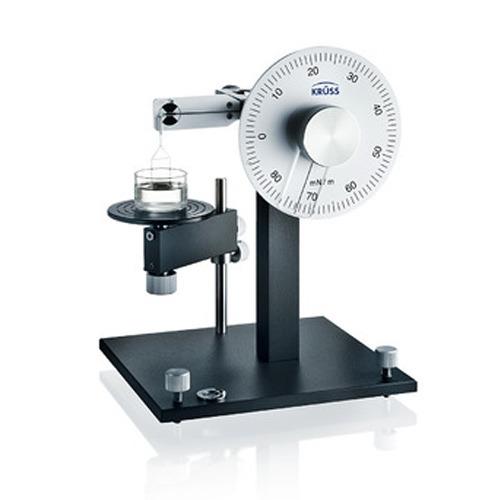
\includegraphics[width=0.7\linewidth]{img/tensiometer}
\caption{Das verwendete Tensiometer}
\label{fig:versuchsaufbau-ebull}
\end{figure}



\section{Ergebnisse}
\label{sec:ergebnisse}
\subsection{Berechnung des Apparatekorrekturfaktors}

Der Apparatekorrekturfaktor K$_{\text{Ka}}$ berechnet sich aus dem Verhältnis des theoretischen Wertes für die Oberflächenspannung des bidestillierten Wasers bei \SI{20}{\degreeCelsius} zum am Tensiometer abgelesenen Wert. Die Berechnung mit den für diesen Versuch gültigen Werten ist in Gleichung \eqref{Kkal} dargestellt. Der abgelesene Wert stammt aus der Messreihe zur Kalibrierung bei \SI{20}{\degreeCelsius}, welche auf dem angehängten Deckblatt zum Versuch einzusehen ist.

\begin{flalign}\label{Kkal}
	\text{K}_{\text{Ka}}&=\frac{\text{theoretischer Wert}}{\text{abgelesener Wert}}\\
	&=\frac{\SI{72,8}{\milli\newton\per\meter}}{\SI{70,0}{\milli\newton\per\meter}}\\
	&=\underline{\underline{1,04}}
\end{flalign}


\subsection{Einwaagen und Volumina der hergestellten Lösungen}

\begin{table}[h!]
	\centering
	\caption{Massen und Volumina der zur Herstellung der Lösungen verwendeten Chemikalien}
	\label{tab:Einwaagen}
	%\resizebox{12.6cm}{!}{
	\begin{tabular}{|c|c|c|c|}
		\hline
	\multirow{ 2}{*}{\textbf{Stoff}} & \textbf{Zielkonzentration } & \textbf{Einwaage}  & \textbf{Volumen} \\ 
		&[\si{\mole\per\liter}]&[\si{\gram}]&[\si{\milli\liter}]\\
		\hline
		Ethanol & 0,1 & - & 0,58\\ 
		Natriumchlorid& 0,1 & 0,58433 &-\\ 
		Natriumdodecylsulfat (\SI{10}{\gram\per\liter})& 0,001& -&0,28\\
		\hline
		
	\end{tabular}
	%	}
\end{table}
\FloatBarrier
\vspace*{-2.5mm}
%Tabelle Ende
\subsection{Korrektur der abgelesenen Oberflächenspannungen}

Die Korrektur der abgelesenen Oberflächenspannungen ($\sigma^\ast$) erfolgt durch die Multiplikation mit dem Apparatekorrekturfaktor (K$_{\text{Ka}}$) und dem Korrekturfaktor nach \textsc{Harkins \& Jordan} (K). Letzterer Korrekturfaktor wurde aus der, der Versuchsanleitung angehängten, Tabelle 01 entnommen. In den Fällen, wo ein Wert nicht passend eingetragen war, wurde der dem gesuchten Wert am nächsten liegende genutzt.

Die Korrekturen erfolgten analog der Rechnung in Gleichung \eqref{korrektur}.

\begin{flalign}\label{korrektur}
	\sigma&=\sigma^\ast*\text{K}_{\text{Ka}}*\text{K}\\
	&=\SI{69,8}{\milli\newton\per\meter}*1,04*0,996\\
	&=\underline{\underline{\SI{72,30}{\milli\newton\per\meter}}}
\end{flalign}

\subsection{Prüfung auf Ausreißer}

Das Kriterium für einen Ausreißer wurde als Abweichung um mehr als die dreifache Standardabweichung vom Mittelwert definiert ($\pm 3*s$). Es wurde ein Ausreißer gefunden. Es handelt sich um den dritten Messwert zum Einfluss des Geschirrspülmittels. Dieser wurde daher gestrichen.

\subsection{Probe auf linearen Zusammenhang}

Durch auftragen der gemessenen und korrigierten Oberflächenspannungen des destillierten Wassers über der Temperatur wird ein Graph erzeugt, welcher es erlaubt, eine Aussage über die Linearität der Messpunkte, zu treffen.

\begin{figure}[h!]
	\begin{center}
		\resizebox{0.8\textwidth}{!}{
			\begin{tikzpicture}[trim axis left, trim axis right]
			\begin{axis}[
			axis lines = left,
			width = 15cm,
			height = 11cm,
			xmin = 0,
			xmax = 67,
			ymin = 66,
			ymax = 74.5,
				ytick = {50,51,...,74},
				xtick = {0,5,...,65},
			ylabel={Oberflächenspannung in \si{\milli \newton \per \meter}},
			%y label style={at={(0,0.5)}},
			xlabel={Temperatur in \si{\celsius}},
			legend style={at={(0.35,0.9)},anchor=west},
			%	y dir = reverse,
			]				
			\addplot [color=black, mark=*] coordinates{(20,72.5) (30,72.198)  (40,70.41) (60,67.19) };
			
			\addplot +[mark=none, dashed, black, domain=15:65] {-0.1400728183*x + 75.830567};
			
			
			
			\legend{gemittelte und korrigierte Oberflächenspannungen, Regressionsgerade $\sigma=-\SI{0,1400}{}*T + \SI{75.83}{} \, | \, R^2$ = \SI{0,962}{}}
			\end{axis}
			\end{tikzpicture}}
		\caption{Oberflächenspannung des Wassers in Abhängigkeit der Temperatur}
		\label{dia:oberflaechenT}
	\end{center}
\end{figure}
\FloatBarrier

Die Geradenparameter der Regressionsgerade der Abbildung \ref{dia:oberflaechenT} sind in Tabelle \ref{tab:ab} eingetragen.

\begin{table}[h!]
	\centering
	\caption{Ermittelte Geradenparameter zur Beschreibung der Oberflächenspannung von Wasser in Abhängigkeit von der Temperatur in \si{\degreeCelsius}}
	\label{tab:ab}
	%\resizebox{12.6cm}{!}{
		\begin{tabular}{|c|c|}
			\hline
			a&-0,1400\\
		\hline
			b&75,8306\\
			\hline
			
		\end{tabular}
	%}
\end{table}
\FloatBarrier
\vspace*{-2.5mm}
%Tabelle Ende

Die Oberflächenspannung des Wassers bei \SI{90}{\degreeCelsius} kann durch Einsetzen in die, aus den Geradenparametern erzeugte Funktion, ermittelt werden. Sie Beträgt \SI{63,23}{\milli\newton\per\meter}. Die Rechnung ist als Gleichung \eqref{gl:90grad} nachfolgend aufgeführt. 

\begin{flalign}\label{gl:90grad}
	\sigma&=-0.1400*T[\si{\degreeCelsius}] + 75.8306\\
	&=-0.1400*90 + 75.8306\\
	&=\underline{\underline{\SI{63,23}{\milli\newton\per\meter}}}
\end{flalign}

\section{Fehlerbetrachtung}
\label{sec:fehler}
Die Ableseungenauigkeit wurde im Kapitel \ref{sec:durchfuerung} bereits angesprochen. Die Nachkommastellen unterliegen daher einer geschätzten Abweichung von $\pm$\SI{0,2}{\milli\newton\per\meter}. Im laufe des Versuches wurde die Apparatur, durch auflegen der Handballen beim vorsichtigen Hantieren an den Stellschrauben, zwei  mal zum Kippeln gebracht. Dabei könnten sich die Einstellungen geringfügig verändert haben. Es waren aber keine Abweichungen festzustellen. Nach jedem Probenwechsel muss einige Zeit gewartet werden, bis der Temperiermantel die Probe gleichmäßig auf die am Thermostat eingestellte Temperatur gebracht hat. Die Einstellung des thermischen Gleichgewichts konnte nur geschätzt werden. Es ist wahrscheinlich, dass mit den Messungen begonnen wurde, bevor das Medium die gewünschte Temperatur hatte. Zur Herstellung der Natriumdodecylsulfatlösung wurde der falsche Ausgangsstoff verwendet. Das Natriumdodecylsulfat setzt sich mit der Zeit am Boden des Gefäßes ab. Aus diesem Grund befindet sich stets eine kleinere Menge auf dem Laborschüttler. In diesem Falle stammte die Reagenz aber aus der Vorratsflasche. Diese wurde nur kurz aufgeschüttelt. Es muss angenommen werden, dass die erhaltene Lösung eine etwas geringere Konzentration aufwies. Des weiteren wurde im Zusammenhang mit den Natriumdodecylsulfat festgestellt, dass verhältnismäßig große Abweichungen zwischen den einzelnen Messergebnissen auftraten. Als entscheidende Einflussgröße auf das Abrissverhalten wurde die Hebegeschwindigkeit des Ringes ermittelt. Je langsamer die Spannung gesteigert wurde, desto geringer war die gemessene Kraft, bei der der Film abriss. Die rundheit des Ringes wirkt sich auf die Messergebnisse aus. Es ist zu beachten, dass der Ring nie ideal kreisförmig sein wird, auch wenn durch Sichtprüfung keine Formfehler festgestellt werden konnten. Im Probengefäß kommen auch Lösungen zum Einsatz. Rückstände selbiger könnten trotz des gründlichen Spülens die nachfolgenden Messungen beeinflusst haben. Die verwendeten Korrekturfaktoren nach \textsc{Harkins \& Jordan} sind aus einer Tabelle abgelesen und nur für die jeweiligen Messwerte angenähert. Die Beschreibung selbiger durch eine Funktion, hätte vermutlich zu präziseren Ergebnissen geführt. Zur Herstellung der Lösungen, hätte die Dosierung der Volumina, durch zusätzliches Einwiegen der Flüssigkeiten, abgesichert werden können. Die Positionierung des Ringes im Probengefäß wirkt sich auch auf das Versuchsergebnis aus. In den Randbereichen unterliegt der Ring auch Wechselwirkungen mit dem Meniskus an der Gefäßwand. Wäre das Gefäß größer dimensioniert, könnte diesem Einfluss besser entgegengewirkt werden.
Die Kalibrierung oder die Korrektur der Messwerte muss fehlerbehaftet sein, weil die korrigierte Oberflächenspannung nicht auf den Erwartungswert von \SI{72,8}{\milli\newton\per\meter} kommt. Es stellt sich heraus dass ein Korrekturfaktor K von 1, anstatt der aus der Tabelle abgelesenen 0,996, zum gewünschten Ergebnis führen würde. Diese Änderung verbessert außerdem den Bestimmtheitsgrad der Regressionsgerade im Kapitel \ref{sec:ergebnisse} 


\section{Diskussion der Ergebnisse}
\label{sec:diskussion}

\subsubsection*{a{)} Warum ist für sehr genaue Messungen eine Korrektur der am Hg-Präzisionsbarometer abgelesenen Druckwerte nötig? Um welche Art von Korrekturen handelt es sich?}
Beim Ablesen am Barometer wird die Länge einer Quecksilbersäule betrachtet. Auf die Länge dieser Säule haben neben dem Luftdruck auch noch andere Faktoren Einfluss. Eine Korrektur des Luftdruckes ist notwendig um diese Faktoren zu kompensieren und damit eine Vergleichbarkeit der Werte zu erzeugen. Die Länge der Skala und das Volumen des Quecksilbers sind Temperaturabhängig. Temperaturschwankungen führen zu Kontraktion und Expansion. Die Korrektur erfolgt durch Umrechnung auf eine Temperatur von \SI{0}{\degreeCelsius}. Die Erdbeschleunigung "`zieht"' je nach Höhe über NN und Breitengrad unterschiedlich an der Quecksilbersäule. Korrekturstandard ist daher der 45. Breitengrad auf Meereshöhe (NN). Zuletzt muss auch der konvexe Quecksilbermenikus berücksichtigt werden welcher innerhalb des Glasrohres entsteht. Die Korrektur wurde in diesem Versuch durch das Computerprogramm BARO ausgeführt. 
\cite{Barometerkorrektur}

\subsubsection*{b{)} Erläutern Sie inwiefern Verunreinigungen in der flüssigen Phase zu einer Fehlbestimmung der temperaturabhängigen Dampfdruckwerte führen können.}
Ist die Probe durch leichtsiedende Stoffe verunreinigt, so wird ein höherer Dampfdruck gemessen. Die verunreinigende Komponente verfälscht mit ihrem höheren Dampfdruck die Messung. Ein alltägliches Beispiel für ein ähnliches System wäre Ethanol in Wasser. Eine zweite Möglichkeit wäre die Kontamination mit einem Salz. Diese hat eine Siedepunktserhöhung zur Folge.\cite{Verunreinigungen}

\subsubsection*{c{)} Stellen Sie Formel und Bedeutung der Clausius-Clapeyron-Gleichung dar und zeigen Sie durch Integration wie daraus die August'sche Dampfdruckgleichung erhalten werden kann.}

Die Clausius-Clapeyron-Gleichung \eqref{gl:CCG} ist ein Sonderfall der Clapeyron-Gleichung und beschreibt den allgemeinen Zusammenhang zwischen Dampfdruck und Temperatur. Sie erlaubt es den Verlauf der Phasengrenze zwischen flüssiger und gasförmiger Phase zu berechnen.

Die Umformung in die August'sche Dampfdruckgleichung hat zwei Annahmen als Voraussetzung. Zum Ersten wird ideales Gasverhalten angenommen. 

\begin{flalign}\label{gl:CCG}
	\frac{dp}{dT}&=\frac{\Delta H_{m,v}}{\Delta V_{m,v}*T}
\end{flalign}
Zum Zweiten wird das molare Volumen der Flüssigkeit gegenüber dem molaren Volumen des Dampfes vernachlässigt \eqref{vernachlassigt}, wodurch für die Änderung des molaren Volumens das molare Volumen des Dampfes eingesetzt werden kann.\eqref{eingesetzt}
\begin{flalign}\label{vernachlassigt}
	\Delta V_{m,v}= \left( V_{m,v}^{Dampf} -  \underbrace{V_{m,v}^{Liquid}}_{\rightarrow\,0}\right)= V_{m,v}^{Dampf}
\end{flalign} 

\begin{flalign}\label{eingesetzt}
	\frac{dp}{dT}&=\frac{\Delta H_{m,v}}{\Delta V_{m,v}^{Dampf}*T}
\end{flalign}

Aufgrund der Annahme des idealen Gasverhaltens, kann nun die ideale Gasgleichung nach dem Volumen umgestellt \eqref{idealesGG} und für das molare Volumen des Dampfes eingesetzt werden.\eqref{allesdrin}

\begin{flalign}\label{idealesGG}
	p*V&=n*R*T\\
	V_{m,v}^{Dampf}=\frac{V}{n}&=\frac{R*T}{p}
\end{flalign}
\begin{flalign}\label{allesdrin}
\frac{dp}{dT}&=\frac{\Delta H_{m,v}*p}{T^2*R}\\ 
\frac{dp}{p}&=\frac{\Delta H_{m,v}}{T^2*R}*dT
\end{flalign}
Es folgt die Integration \eqref{int} des Ausdruckes zur August'schen Dampfgleichung \eqref{august}.
\begin{flalign}\label{int}
	\int\frac{dp}{p}&=\int\frac{\Delta H_{m,v}}{T^2*R}*dT
\end{flalign}
\begin{flalign}\label{august}
	\ln\left( \frac{p_2}{p_1}\right)&=\frac{\Delta H_{m,v}}{R}* \left(\frac{1}{T2}-\frac{1}{T1}\right)
\end{flalign}
\subsubsection*{d{)} Wie können Sie graphisch prüfen, dass der Dampfdruck einer reinen Flüssigkeit unter Annahme idealen Verhaltens für die Gas- Flüssigkeitsphase eine exponentielle Temperaturabhängigkeit besitzt?}

Die exponentielle Temperaturabhängigkeit kann gepfüft werden, in dem eine Exponentialfunktion für die gefundenen Messpunkte angenähert wird. Für den Dampfdruck kann dies über die \textit{ANTOINE}-Gleichung geschehen. Für den Dampfdruck des reinen Isopropanols, unter Annahme idealen Verhaltens, ist der exponentielle Zusammenhang aus der Form der entsprechend umgestellten \textit{ANTOINE}-Gleichung \ref{sec:berechnungDampfdruckkurveausKonstanten} ersichtlich. Den endgültigen Beweis erbringt ein Blick in die Abb.\ref{dia:p/Tmess}, wo bereits erwähnte Exponentialgleichung eingetragen ist. Die Druckmesspunkte liegen praktisch auf der Exponentialfunktion und belegen so die exponentielle Temperaturabhängigkeit. 


\subsubsection*{e{)} Wofür steht am Präzisionsthermometer der Begriff Pt-100? Erläutern sie kurz das dahinterstehende Messprinzip der Temperaturbestimmung}

Die Bezeichnung Pt-100 steht für einen Platinwiderstand mit \SI{100}{\ohm}. Der elektrische Widerstand eines Leiters ändert sich mit der Temperatur. Metalle, wie auch Platin eines ist, verringern ihre Leitfähigkeit mit Steigender Temperatur, wodurch sich ihr Widerstand erhöht. Durch Messung dieses Ohm'schen Widerstandes kann anhand einer Kalibrierung auf die Temperatur des Metalls geschlossen werden.\cite{Widerstandsthermometer}

\subsubsection*{f{)} Stellen Sie die bestimmten Dampfdruckwerte als Funktion der Temperatur in einem Diagramm dar.}

Die Darstellung ist als Abb.\ref{dia:p/Tmess} im Kapitel \ref{sec:ergebnisse} zu finden.

\subsubsection*{g{)} Erstellen Sie auf Basis ihrer Daten ein zweites Diagramm, in dem der natürliche Logarithmus des Dampfdrucks gegen die inverse Temperaturaufgetragen wird. Diskutieren Sie das Ergebnis im Hinblick auf die August'sche Dampfgleichung und beurteilen Sie die Linearität mit einer geeigneten Kenngröße. Ermitteln Sie darüber hinaus aus dem Geradenanstieg die molare Verdampfungsenthalpie $\Delta_{LV}H_m$ des untersuchten Stoffes. Vergleichen Sie mit dem entsprechenden Literaturwert und diskutieren Sie mögliche Ursachen für ggf. vorhandene Abweichungen.}

Die geforderte Darstellung ist im Kapitel \ref{sec:ergebnisse} als Abb. \ref{dia:lnp/1/T} zu finden. Als Kenngröße für die Linearität wurde das Bestimmtheitsmaß der Regressionsgerade durch die Punkte aus den Wertepaaren gewählt. Dieses Bestimmtheitsmaß wird vom Tabellenkalkulationsprogramm \textsc{Libre-Office Calc} mit einem Betrag von rund 0.99985 angegeben. Dieser Wert ist sehr nah an der 1, was bedeutet, dass die gefundene Regressionsgerade sehr nah an den Punkten aus den Wertepaaren liegt. Die Linearität ist als sehr hoch einzustufen. 

Die Berechnung der molaren Verdampfungsenthalpie ist im Kapitel \ref{sec:berechnungMolareVerdEnthalpie} zu finden. Aus dem Geradenanstieg ergab sich dabei eine molare Verdampfungsenthalpie des Isopropanols von rund \SI{43,5}{\kilo\joule\per\mole}. In der Literatur \cite{molareVerdampfungsenthalpieLiteraturwert} findet sich im Vergleich dazu eine molare Verdampfungsenthalpie von \SI{39,85 }{\kilo\joule\per\mole}. Der im Experiment ermittelte Wert liegt ein Wenig über dem Literaturwert. Gründe dafür sind in den Annahmen zur Berechnung zu suchen. Es wurde ein reales System untersucht. Ein solches kann sich nie vollkommen ideal verhalten. Das molare Volumen der Flüssigkeit mag zwar klein sein, aber trotzdem existiert es. Bei einer jeden Messung können systematische und zufällige Fehler Einfluss auf das Ergebnis nehmen. Näheres zu den Fehlern ist im Kapitel \ref{sec:fehler} aufgeführt.
\subsubsection*{h{)} Mit Hilfe eines Datenauswerte-Programms, wie Excel oder ZUST, ist für die gemessenen Wertepaare p$^\circ$-T eine Regressionsrechnung durchzuführen. Dabei sind die Konstanten A, B und C der \textit{ANTOINE}-Gleichung zu bestimmen und mit Literaturwerten zu Vergleichen.}

Die durch das Programm \textsc{ZUST} aus den experimentellen Daten ermittelten \textit{ANTOINE}\--Konstanten sind in der Spalte "`Experimentell"' der Tab.\ref{tab:AntoineKonstanten} eingetragen. Die ebenfalls aus dem Programm ZUST entnommenen Literaturwerte sind nebenstehend in der Spalte "`Literatur"' dargestellt. Die Literaturwerte sind deutlich höher als die im Experiment ermittelten Konstanten. Diese Abweichung kann auf den unterschiedlichen Geltungsbereich zurückzuführen sein. Die Literaturwerte gelten für einen um \SI{60}{\kelvin} weiteren Temperaturbereich als die experimentell bestimmten Werte. Das ist weit mehr als das Doppelte und relativiert eine maximale Abweichung von ca. 30\%.

\begin{table}[h!]
	\centering
	\caption{Gegenüberstellung der experimentell ermittelten \textit{ANTOINE}-Konstanten mit Literaturwerten, sowie die zugehörigen Geltungsbereiche}
	\label{tab:AntoineKonstanten}
	%\resizebox{12.6cm}{!}{
	\begin{tabular}{|c|c|c|}
		\hline
			\textbf{Konstante} & \textbf{Experimentell} & \textbf{Literatur} \\ 
			\hline
			A & 6,933 & 8,003 \\ 
			B & 1396,28 & 2010,33 \\ 
			C & 201,633 & 252,635\\
		\hline
		\hline
		T$_\text{Lo}$ [\si{\degreeCelsius}]&33,7&-25\\
	T$_\text{Hi}$ [\si{\degreeCelsius}]	&81,4&83\\
	\hline
	\end{tabular}
	%	}
\end{table}
\FloatBarrier
\vspace*{-2.5mm}
%Tabelle Ende
\subsubsection*{i{)} Nutzen Sie ihre ermittelten \textit{ANTOINE}-Parameter, um die p$^\circ$-T-Dampfdruckkurve mit der \textit{ANTOINE}-Gleichung zu berechnen und vergleichen Sie ihre experimentellen Werte mit den berechneten Werten im Diagramm.}
Die Dampfdruckkurve aus den berechneten \textit{ANTOINE}-Parametern ist in der Abb. \ref{dia:p/Tmess} eingetragen. Die \textit{ANTOINE}-Gelichung mit eingesetzten Parametern ist im Kapitel \ref{sec:berechnungDampfdruckkurveausKonstanten} als Gl. (\ref{gl:antoineEingesetzt}) dargestellt. Die experimentellen Werte liegen alle sehr nah an dem berechneten Graphen. Die gefundenen \textit{ANTOINE}-Parameter beschreiben den im Experiment beobachteten Zusammenhang exakt.

\section{Zusammenfassung und Fazit}
\label{sec:zusammenfassung}

Die experimentellen Messdaten kommen sehr nah an die Literaturwerte heran, wie aus \ref{dia:p/Tmess} hervorgeht. Das Verhalten des Isopropanols kann sehr exakt durch die Antoine-Gleichung ausgedrückt werden. Teilweise waren die Literaturwerte zum Vergleich wenig geeignet. Das erschwert die Einschätzung. Die Verwendung der Computerprogramme ZUST und BARO ermöglichte sehr präzise und belastbare Berechnungen. Noch aussagekräftigere Ergebnisse hätten durch eine mehrfach wiederholte Messung erhalten werden können. Auch eine kleinere Schrittweite bei der Einstellung der Drücke wäre sinnvoll, um sich noch genauer an die Realität anzunähern. Von Extrapolationen über den untersuchten Bereich hinaus ist dringend abzuraten.

%Praktikumsskript, Modul ………, Versuch …….., Prof. Musterprof. 
%DIN 12345, Jahr der Veröffentlichung 
%Link der Internetseite, Zugriffsdatum 
%Buchtitel, Autor, Verlag, Veröffentlichungsjahr 

%Literaturverzeichnis Bücher
\bibliography{Literatur}
\bibliographystyle{unsrtdin}
\addcontentsline{toc}{section}{Literaturverzeichnis}



\section*{Anhang}
\addcontentsline{toc}{section}{Anhang}
\label{sec:anhang}

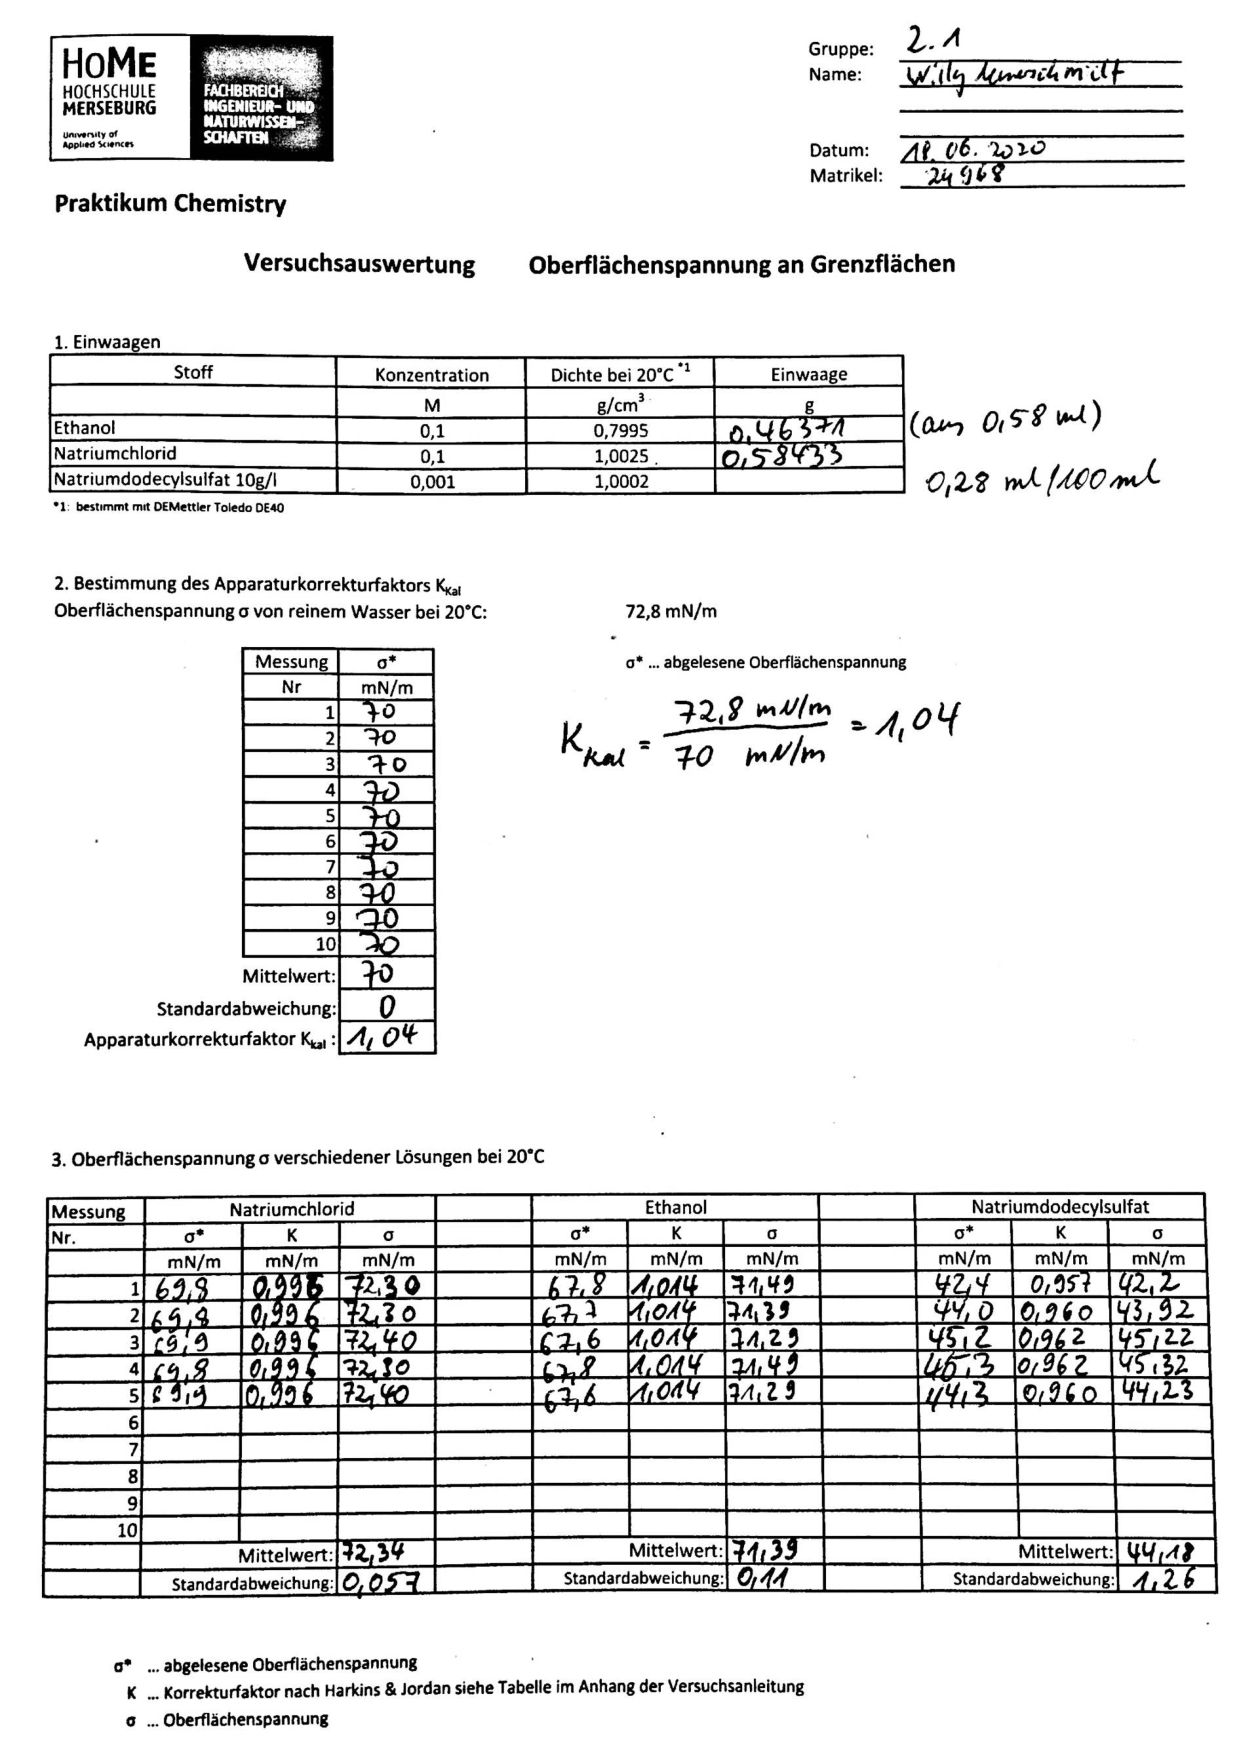
\includepdf[pages=1-2]{deckblatt}

%\chapter*{Eidesstattliche Erklärung}
\label{erklaerung}
Hiermit versichere ich, die vorliegende Seminararbeit selbstständig und nur unter Verwendung der von mir angegebenen Quellen und Hilfsmittel verfasst zu haben. Sowohl inhaltlich als auch wörtlich entnommene Inhalte wurden als solche kenntlich gemacht. Die Arbeit hat in dieser oder vergleichbarer Form noch keinem anderem Prüfungsgremium vorgelegen. \\
\\[1.5cm]
Datum:	\hrulefill\enspace Unterschrift: \hrulefill
\\[3.5cm]
\addcontentsline{toc}{chapter}{Selbstständigkeitserklärung}

\end{document}
